\newpage
\section{Transformations on point clouds (2)}

\subsection{Aligning the training and testing data}

\Cref{code:task_3_1} shows the code I use to compute the alignments, and
\cref{fig:task_3_1} shows the alignments of the first ten training wings using
the first training wing as target.


\emph{Please note:} The assignment text states that ``\emph{The landmark points
[...] can be visualized as closed curves, which we will do in these
questions}'', however Figure 1 in the assignment text shows the landmarks
plotted with a scatter plot. Hence it is ambiguous as to whether the aligned
wings should be plotted using a scatter plot or as a closed curve. I choose to
plot the closed curves even if the plots are a little messy.

\begin{figure}[H]
  \centering
  \begin{minted}[fontsize=\footnotesize]{python}
from scipy.spatial import procrustes
...
def procrustes_many(target_wing, wings):
    return np.array([procrustes(target_wing, wing)[1]
                     for wing in wings])
...
# perform procrustes.
target_wing = train_wings[0]
train_wings_aligned = procrustes_many(target_wing, train_wings)
test_wings_aligned  = procrustes_many(target_wing, test_wings)
  \end{minted}
  \captionof{listing}{Code for Procrustes alignment of training and testing data.}
  \label{code:task_3_1}
\end{figure}

\begin{figure}[H]
  \centering
  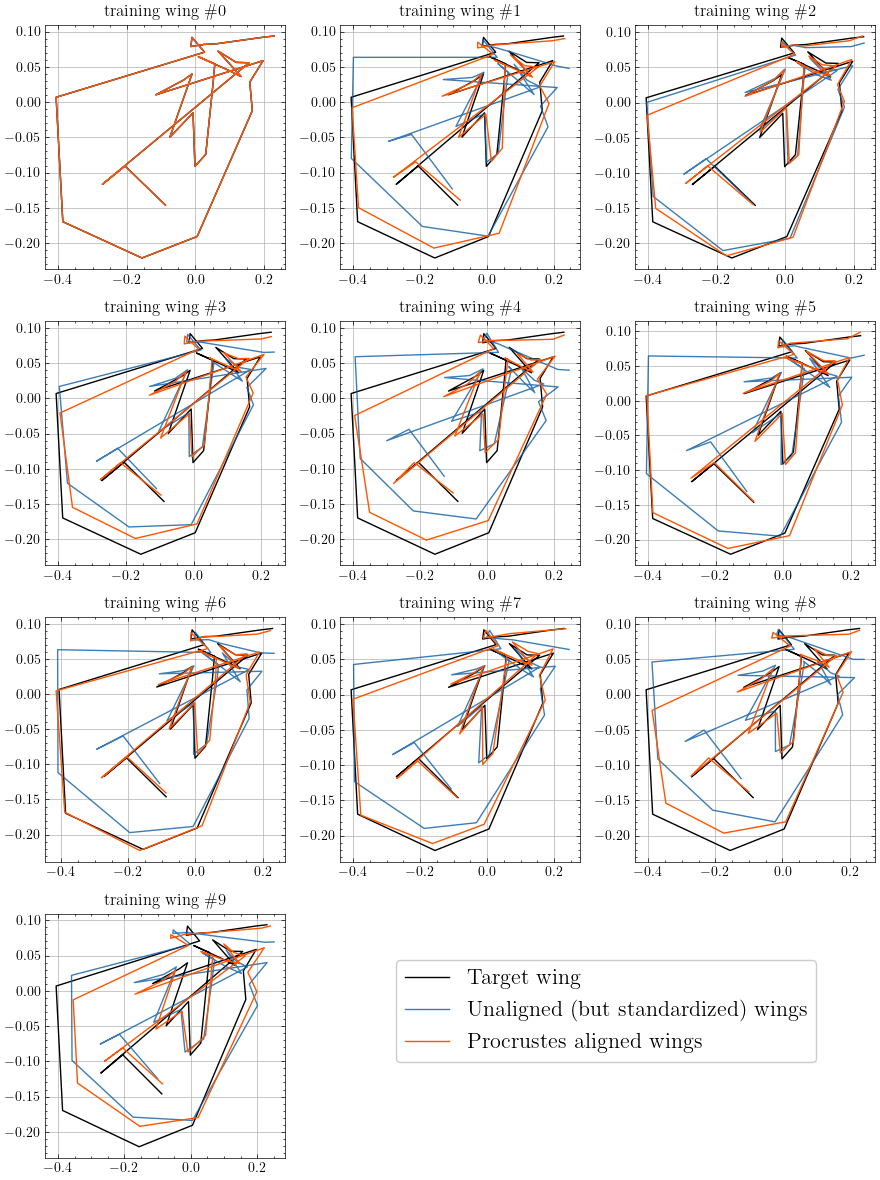
\includegraphics[width=\textwidth]{figures/task_3_1.png}
  \caption{Procrustes alignments of the first 10 training wings using the first
  training wing as target.}
  \label{fig:task_3_1}
\end{figure}

\subsection{Alignment and classification}

I choose to simply use a k-NN classifier to perform the classifications, and I
use the implementation from \texttt{sklearn} with uniformly weighted neighbors.

I perform a simple parameter search to find the optimal value for $k$ for both
the unaligned and aligned training data sets. The parameter search uses a
randomly generated 20\% training/validation split.

I find $k = 3$ and $k = 1$ to be optimal for the unaligned and aligned training
sets, respectively, and the prediction accuracies obtained were $\simeq 0.519$
and $\simeq 0.937$ for the unaligned and aligned testing data, respectively.

\emph{To reproduce the results as well as the parameter search, please run
\texttt{task\_3\_2()} in the attached \texttt{task\_3.py}.}

As expected, the classifier performed better on the aligned data, mispredicting
only roughly 1 out of 20 cases, as opposed to the unaligned data where we
saw mispredictions in roughly half of cases.

\subsection{Loss of information in Procrustes}

When we perform Procrustes, the standardization preserves only the handedness,
relative position of landmarks, etc., but removes information about the relative
sizes of the wings between different species of flies and different samples in
the dataset. This means that predictions are made based on shape and relative
distance between pairs of landmark points.

When it comes to classification, this is only a big problem if there exists two
or more species of flies for which the wings are similar in all but the size --
in other words, if the distinguishing feature happens to be the size, not the
shape.

To examine whether this \emph{could} be a potential source of error for this
particular data set, we can examine the mean size of the wing samples across
each species. Figure \cref{fig:wing_lens} shows the mean wing size for each
species, where wing size is quantified by measuring the length of the closed
curve given by the points in a wing sample.

From the plot we see that three of the 15 species are outliers when it comes to
the mean wing size -- namely the albizona, tecticauda, and warreni species --
and that 30 out of the total 261 samples belong to these classes. This number is
not so high that I expect it to outweigh the benefits in accuracy obtained from
Procrustes.

\emph{However, please note that two species for which the mean wing size is very
different may still be easily distinguishable from one another after
standardization if, as explained, they are also different in
features/landmarks.}

\begin{figure}[H]
  \centering
  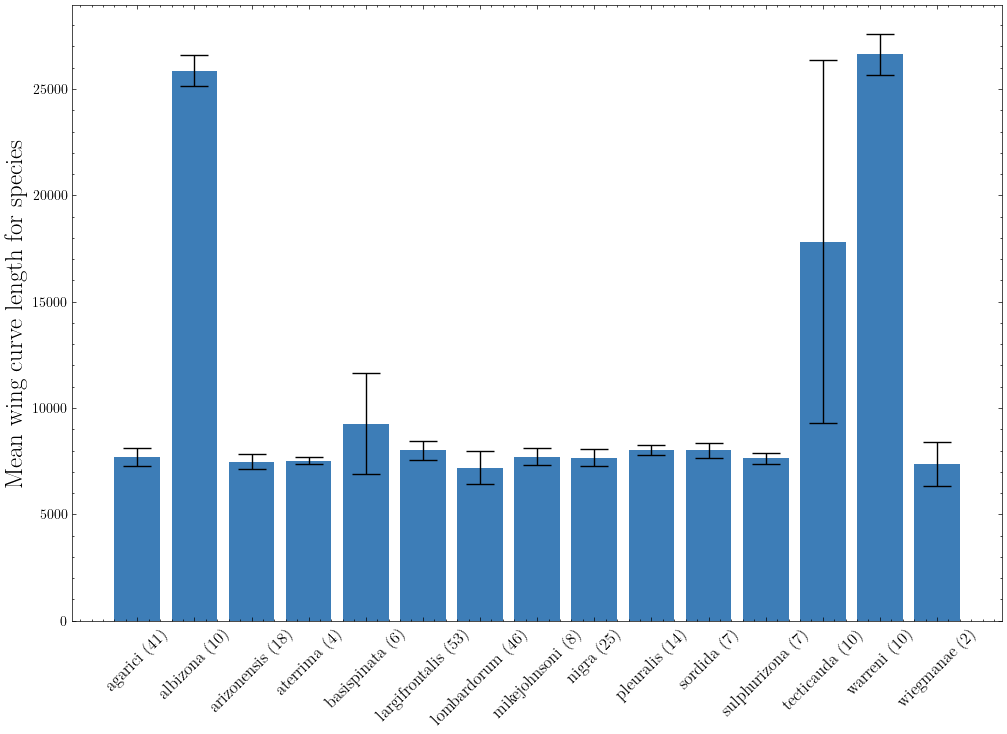
\includegraphics[width=\textwidth]{figures/task_3_wing_lens.png}
  \caption{Mean wing curve length for each species measured on the combined
  training and test sets. The number in parentheses after each species name is
  the number of samples belonging to that species.}
  \label{fig:wing_lens}
\end{figure}
